% Options for packages loaded elsewhere
% Options for packages loaded elsewhere
\PassOptionsToPackage{unicode}{hyperref}
\PassOptionsToPackage{hyphens}{url}
\PassOptionsToPackage{dvipsnames,svgnames,x11names}{xcolor}
%
\documentclass[
  8pt,
  a4paper]{article}
\usepackage{xcolor}
\usepackage[lmargin=2cm,rmargin=2cm,tmargin=2cm,bmargin=2cm]{geometry}
\usepackage{amsmath,amssymb}
\setcounter{secnumdepth}{-\maxdimen} % remove section numbering
\usepackage{iftex}
\ifPDFTeX
  \usepackage[T1]{fontenc}
  \usepackage[utf8]{inputenc}
  \usepackage{textcomp} % provide euro and other symbols
\else % if luatex or xetex
  \usepackage{unicode-math} % this also loads fontspec
  \defaultfontfeatures{Scale=MatchLowercase}
  \defaultfontfeatures[\rmfamily]{Ligatures=TeX,Scale=1}
\fi
\usepackage{lmodern}
\ifPDFTeX\else
  % xetex/luatex font selection
\fi
% Use upquote if available, for straight quotes in verbatim environments
\IfFileExists{upquote.sty}{\usepackage{upquote}}{}
\IfFileExists{microtype.sty}{% use microtype if available
  \usepackage[]{microtype}
  \UseMicrotypeSet[protrusion]{basicmath} % disable protrusion for tt fonts
}{}
\makeatletter
\@ifundefined{KOMAClassName}{% if non-KOMA class
  \IfFileExists{parskip.sty}{%
    \usepackage{parskip}
  }{% else
    \setlength{\parindent}{0pt}
    \setlength{\parskip}{6pt plus 2pt minus 1pt}}
}{% if KOMA class
  \KOMAoptions{parskip=half}}
\makeatother
% Make \paragraph and \subparagraph free-standing
\makeatletter
\ifx\paragraph\undefined\else
  \let\oldparagraph\paragraph
  \renewcommand{\paragraph}{
    \@ifstar
      \xxxParagraphStar
      \xxxParagraphNoStar
  }
  \newcommand{\xxxParagraphStar}[1]{\oldparagraph*{#1}\mbox{}}
  \newcommand{\xxxParagraphNoStar}[1]{\oldparagraph{#1}\mbox{}}
\fi
\ifx\subparagraph\undefined\else
  \let\oldsubparagraph\subparagraph
  \renewcommand{\subparagraph}{
    \@ifstar
      \xxxSubParagraphStar
      \xxxSubParagraphNoStar
  }
  \newcommand{\xxxSubParagraphStar}[1]{\oldsubparagraph*{#1}\mbox{}}
  \newcommand{\xxxSubParagraphNoStar}[1]{\oldsubparagraph{#1}\mbox{}}
\fi
\makeatother


\usepackage{longtable,booktabs,array}
\usepackage{calc} % for calculating minipage widths
% Correct order of tables after \paragraph or \subparagraph
\usepackage{etoolbox}
\makeatletter
\patchcmd\longtable{\par}{\if@noskipsec\mbox{}\fi\par}{}{}
\makeatother
% Allow footnotes in longtable head/foot
\IfFileExists{footnotehyper.sty}{\usepackage{footnotehyper}}{\usepackage{footnote}}
\makesavenoteenv{longtable}
\usepackage{graphicx}
\makeatletter
\newsavebox\pandoc@box
\newcommand*\pandocbounded[1]{% scales image to fit in text height/width
  \sbox\pandoc@box{#1}%
  \Gscale@div\@tempa{\textheight}{\dimexpr\ht\pandoc@box+\dp\pandoc@box\relax}%
  \Gscale@div\@tempb{\linewidth}{\wd\pandoc@box}%
  \ifdim\@tempb\p@<\@tempa\p@\let\@tempa\@tempb\fi% select the smaller of both
  \ifdim\@tempa\p@<\p@\scalebox{\@tempa}{\usebox\pandoc@box}%
  \else\usebox{\pandoc@box}%
  \fi%
}
% Set default figure placement to htbp
\def\fps@figure{htbp}
\makeatother





\setlength{\emergencystretch}{3em} % prevent overfull lines

\providecommand{\tightlist}{%
  \setlength{\itemsep}{0pt}\setlength{\parskip}{0pt}}



 


\makeatletter
\@ifpackageloaded{tcolorbox}{}{\usepackage[skins,breakable]{tcolorbox}}
\@ifpackageloaded{fontawesome5}{}{\usepackage{fontawesome5}}
\definecolor{quarto-callout-color}{HTML}{909090}
\definecolor{quarto-callout-note-color}{HTML}{0758E5}
\definecolor{quarto-callout-important-color}{HTML}{CC1914}
\definecolor{quarto-callout-warning-color}{HTML}{EB9113}
\definecolor{quarto-callout-tip-color}{HTML}{00A047}
\definecolor{quarto-callout-caution-color}{HTML}{FC5300}
\definecolor{quarto-callout-color-frame}{HTML}{acacac}
\definecolor{quarto-callout-note-color-frame}{HTML}{4582ec}
\definecolor{quarto-callout-important-color-frame}{HTML}{d9534f}
\definecolor{quarto-callout-warning-color-frame}{HTML}{f0ad4e}
\definecolor{quarto-callout-tip-color-frame}{HTML}{02b875}
\definecolor{quarto-callout-caution-color-frame}{HTML}{fd7e14}
\makeatother
\makeatletter
\@ifpackageloaded{caption}{}{\usepackage{caption}}
\AtBeginDocument{%
\ifdefined\contentsname
  \renewcommand*\contentsname{Table of contents}
\else
  \newcommand\contentsname{Table of contents}
\fi
\ifdefined\listfigurename
  \renewcommand*\listfigurename{List of Figures}
\else
  \newcommand\listfigurename{List of Figures}
\fi
\ifdefined\listtablename
  \renewcommand*\listtablename{List of Tables}
\else
  \newcommand\listtablename{List of Tables}
\fi
\ifdefined\figurename
  \renewcommand*\figurename{\textbf{Figure}}
\else
  \newcommand\figurename{\textbf{Figure}}
\fi
\ifdefined\tablename
  \renewcommand*\tablename{\textbf{Table}}
\else
  \newcommand\tablename{\textbf{Table}}
\fi
}
\@ifpackageloaded{float}{}{\usepackage{float}}
\floatstyle{ruled}
\@ifundefined{c@chapter}{\newfloat{codelisting}{h}{lop}}{\newfloat{codelisting}{h}{lop}[chapter]}
\floatname{codelisting}{Listing}
\newcommand*\listoflistings{\listof{codelisting}{List of Listings}}
\makeatother
\makeatletter
\makeatother
\makeatletter
\@ifpackageloaded{caption}{}{\usepackage{caption}}
\@ifpackageloaded{subcaption}{}{\usepackage{subcaption}}
\makeatother
\usepackage{bookmark}
\IfFileExists{xurl.sty}{\usepackage{xurl}}{} % add URL line breaks if available
\urlstyle{same}
\hypersetup{
  pdftitle={Darwin Harbour Water Quality monitoring program analysis application manual},
  pdfauthor={Murray Logan},
  colorlinks=true,
  linkcolor={blue},
  filecolor={Maroon},
  citecolor={Blue},
  urlcolor={Blue},
  pdfcreator={LaTeX via pandoc}}


\title{Darwin Harbour Water Quality monitoring program analysis
application manual}
\author{Murray Logan}
\date{16/05/2025}
\begin{document}
\maketitle

\renewcommand*\contentsname{Table of contents}
{
\hypersetup{linkcolor=}
\setcounter{tocdepth}{3}
\tableofcontents
}

\section{About}\label{about}

This document comprises the manual for the Darwin Harbour Water Quality
monitoring program analysis application. It provides information on:

\begin{itemize}
\tightlist
\item
  a broad overview of the structure of the application
\item
  the application dependencies and how to install them
\item
  starting the application
\item
  progressing through the analysis pipeline
\item
  visualising, interpreting and extracting outputs
\end{itemize}

\section{Structural overview}\label{structural-overview}

\href{https://www.r-project.org/}{R Graphical and Statistical
Environment} offers an ideal platform for developing and running complex
statistical analyses as well as presenting the outcomes via professional
graphical/tabular representations. As a completely scripted language it
also offers the potential for both full transparency and
reproducibility. Nevertheless, as the language, and more specifically
the extension packages are community developed and maintained, the
environment evolves over time. Similarly, the underlying operating
systems and programs on which R and its extension packages depend
(hereafter referred to as the \emph{operating environment}) also change
over time. Consequently, the stability and reproducibility of R codes
have a tendency to change over time.

\subsection{Docker containers}\label{docker-containers}

One way to attempt to future proof a codebase that must be run upon a
potentially unpredictable operating environment is to
\textbf{containerise} the operating environment, such that it is
preserved to remain unchanged over time. Containers (specifically
\href{https://www.docker.com/}{docker} containers) are lightweight
abstraction units that encapsulate applications and their dependencies
within standardized, self-contained execution environments. Leveraging
containerization technology, they package application code, runtime,
libraries, and system tools into isolated units (\emph{containers}) that
abstract away underlying infrastructure differences, enabling consistent
and predictable execution across diverse computing platforms.

Containers offer several advantages, such as efficient resource
utilization, rapid deployment, and scalability. They enable developers
to build, test, and deploy applications with greater speed and
flexibility. Docker containers have become a fundamental building block
in modern software development, enabling the development and deployment
of applications in a consistent and predictable manner across various
environments.

\subsection{Shiny applications}\label{shiny-applications}

\href{https://shiny.posit.co/}{Shiny} is a web application framework for
R that enables the creation of interactive and data-driven web
applications directly from R scripts. Developed by
\href{https://posit.co/}{Rstudio}, Shiny simplifies the process of
turning analyses into interactive web-based tools without the need for
extensive web development expertise.

What makes Shiny particularly valuable is its seamless integration with
R, allowing statisticians and data scientists to build and deploy
bespoke statistical applications, thereby making data visualization,
exploration, and analysis accessible to a broader audience. With its
interactive and user-friendly nature, Shiny serves as a powerful tool
for sharing insights and engaging stakeholders in a more intuitive and
visual manner. \#\# Git and github

Git, a distributed version control system, and
\href{https://github.com/}{GitHub}, a web-based platform for hosting and
collaborating on Git repositories, play pivotal roles in enhancing
reproducibility and transparency in software development. By tracking
changes in source code and providing a centralized platform for
collaborative work, Git and GitHub enable developers to maintain a
detailed history of code alterations. This history serves as a valuable
asset for ensuring the reproducibility of software projects, allowing
users to trace and replicate specific versions of the codebase.

GitHub Actions (an integrated workflow automation feature of GitHub),
automates tasks such as building, testing, and deploying applications
and artifacts. Notably, through workflow actions, GitHub Actions can
build docker containers and act as a container registry. This
integration enhances the overall transparency of software development
workflows, making it easier to share, understand, and reproduce projects
collaboratively.

Figure~\ref{fig-diagram} provides a schematic overview of the
relationship between the code produced by the developer, the Github
cloud repositiory and container registry and the shiny docker container
run by user.

\begin{figure}

\centering{

\pandocbounded{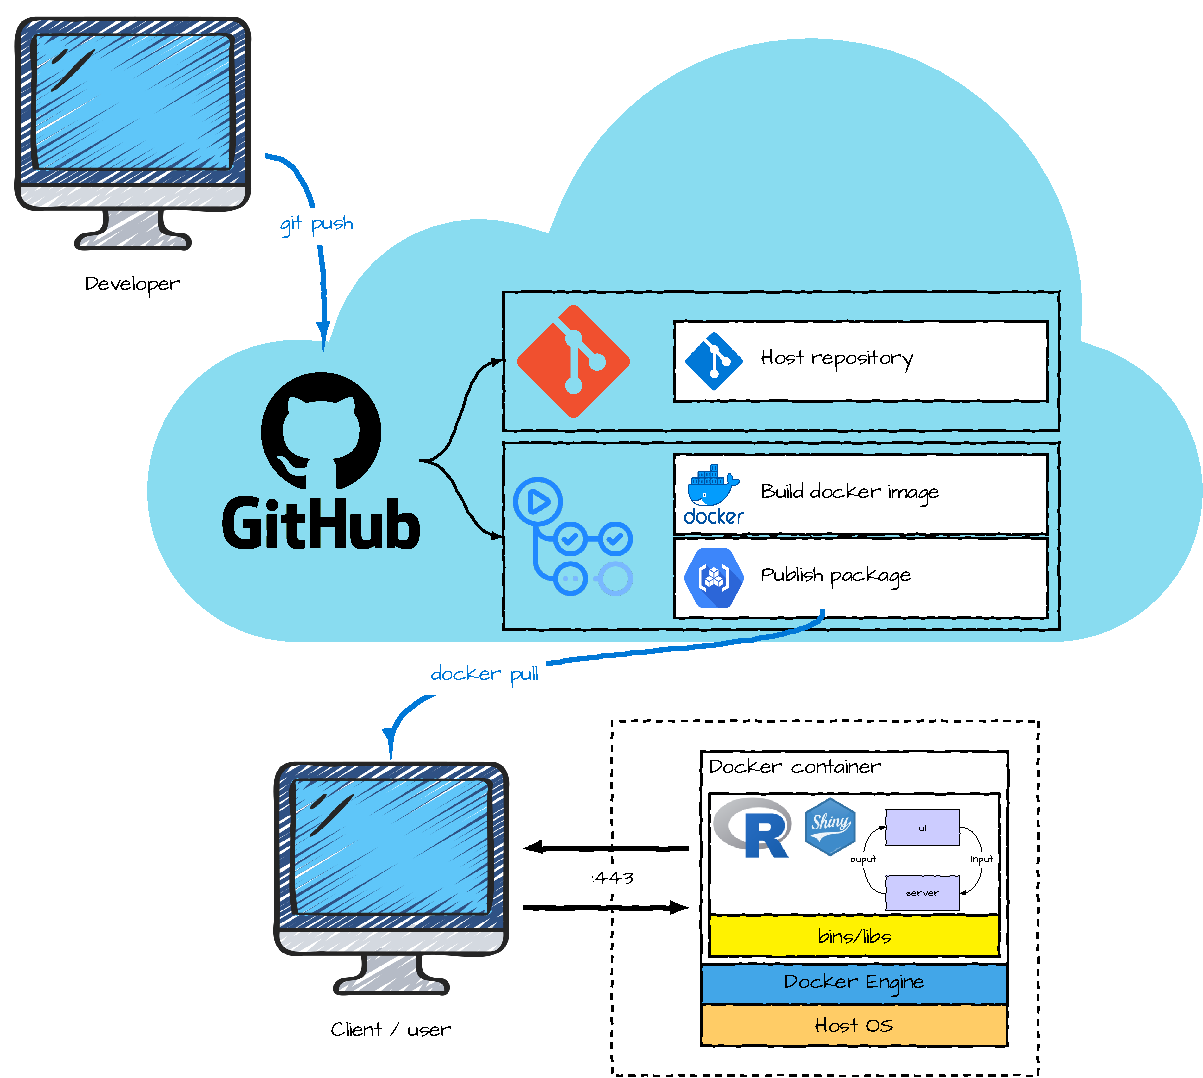
\includegraphics[keepaspectratio]{manual_files/figure-pdf/fig-diagram-1.pdf}}

}

\caption{\label{fig-diagram}Diagram illustrating the relationship
between the code produced by the developer and the shiny docker
container utilised by user with a Github cloud conduit. The developed
codebase includes a Shiny R application with R backend,
\texttt{Dockerfile} (instructions used to assemble a full operating
environment) and github workflow file (instructions for building and
packaging the docker image on github via \texttt{actions}).}

\end{figure}%

\section{Installation}\label{installation}

\subsection{Installing docker desktop}\label{installing-docker-desktop}

To retrieve and run docker containers requires the installation of
\href{https://www.docker.com/products/docker-desktop/}{Docker Desktop}
on Windows and MacOSx

\subsubsection{Windows}\label{windows}

The steps for installing Docker Desktop are:

\begin{itemize}
\item
  \textbf{Download the Installer:} head to
  \url{https://docs.docker.com/desktop/install/windows-install/} and
  follow the instructions for downloading the appropriate installer for
  your Windows version (Home or Pro).
\item
  \textbf{Run the Installer:} double-click the downloaded file and
  follow the on-screen instructions from the installation wizard. Accept
  the license agreement and choose your preferred installation location.
\item
  \textbf{Configure Resources (Optional):} Docker Desktop might suggest
  allocating some system resources like CPU and memory. These settings
  can be adjusted later, so feel free to use the defaults for now.
\item
  \textbf{Start the Docker Engine:} once installed, click the ``Start
  Docker Desktop'' button. You may see a notification in the taskbar -
  click it to confirm and allow Docker to run in the background.
\item
  \textbf{Verification:} open a terminal (or Powershell) and run
  \texttt{docker\ -\/-version}. If all went well, you should see
  information about the installed Docker Engine version.
\end{itemize}

Additional Tips:

\begin{itemize}
\tightlist
\item
  Ensure Hyper-V (virtualization) is enabled in your BIOS settings for
  optimal performance.
\end{itemize}

\subsection{Installing the and running the
app}\label{installing-the-and-running-the-app}

The task of installing and running the app is performed via a single
\textbf{deploy script} (\texttt{deploy\_wq.bat} on Windows or
\texttt{deploy\_wq.sh} on Linux/MacOSX/wsl). For this to work properly,
the deploy script should be placed in a folder along with two additional
folders (one called \texttt{input} and the other called
\texttt{parameters}) that contains the input datasets (in csv format)
and run time parameters. This structure is illustrated below for
Windows.

\begin{verbatim}
\
|- deploy_wq.bat
|- input
   |- 16_wq.csv
   |- 17_wq.csv
   |- overwrites.csv
   |- weights_m.csv
   |- weights_s.csv
|- parameters
   |- config.ini
   |- water_quality_guidelines.csv
   |- spatial.csv
   |- GIS
      |- RCZ_rev24.*
      |- SBZone_upper.*
      |- Middle_Harbour_Upper.*
\end{verbatim}

\begin{tcolorbox}[enhanced jigsaw, leftrule=.75mm, left=2mm, toprule=.15mm, colbacktitle=quarto-callout-note-color!10!white, rightrule=.15mm, breakable, arc=.35mm, opacityback=0, toptitle=1mm, title=\textcolor{quarto-callout-note-color}{\faInfo}\hspace{0.5em}{Note}, titlerule=0mm, coltitle=black, colback=white, opacitybacktitle=0.6, colframe=quarto-callout-note-color-frame, bottomrule=.15mm, bottomtitle=1mm]

In the above illustration, there are two example water quality datasets
(\texttt{16\_wq.csv} and \texttt{17\_wq.csv}). To ensure that the
application correctly identifies them as water quality datasets, it is
important that they are named according to the following format:
\texttt{\textless{}yy\textgreater{}\_wq.csv} where the
\texttt{\textless{}yy\textgreater{}} represents a two digit year
(e.g.~16 for 2016). For additional information on the contents of these
files, please see \textbf{?@sec-data-requirements}.

\end{tcolorbox}

To set up the above structure:

\begin{enumerate}
\def\labelenumi{\arabic{enumi}.}
\item
  create a new folder on your computer in a location of your choice that
  you are likely to remember and easily locate (e.g.~on the desktop).
  Whilst the name of the folder is not important, it is recommended that
  it be named after the project (e.g.
  \texttt{darwin\_harbour\_sediment\_monitoring}).
\item
  download the deploy script from the projects github repository

  \begin{enumerate}
  \def\labelenumii{\alph{enumii}.}
  \item
    go to the projects github repository
    (\url{https://github.com/open-AIMS/dh_wq_monitoring.git}) in a
    browser
  \item
    click on either the \texttt{deploy\_wq.bat} (Windows) or
    \texttt{deploy\_wq.sh} (Linux/MacOSX/wsl).

    \pandocbounded{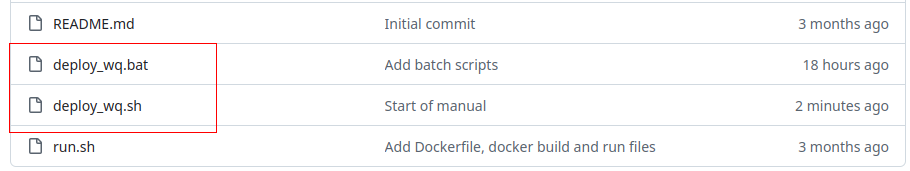
\includegraphics[keepaspectratio]{resources/github_deploy_script.png}}
  \item
    click on the download button and select the project folder as the
    location to download the file to. If the file is automatically
    downloaded to a downloads folder, move the file to the project
    folder.

    \pandocbounded{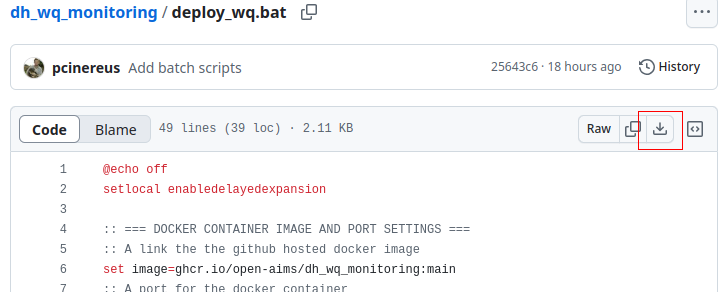
\includegraphics[keepaspectratio]{resources/github_deploy_script2.png}}
  \end{enumerate}
\item
  within the project folder, create folders called \texttt{inputs} and
  \texttt{parameters} (as outlined above) and place all the appropriate
  data sets into these folders
\end{enumerate}

To run the app, navigate inside of the project folder and run (typically
double click) on the deploy script. Upon doing so, you will be presented
with a directory selection window that is prompting for the path of the
project folder. Navigate to and select the project folder before
clicking the ``OK'' button. Shortly thereafter, the application will
appear in a browser tab.

\begin{tcolorbox}[enhanced jigsaw, leftrule=.75mm, left=2mm, toprule=.15mm, colbacktitle=quarto-callout-note-color!10!white, rightrule=.15mm, breakable, arc=.35mm, opacityback=0, toptitle=1mm, title=\textcolor{quarto-callout-note-color}{\faInfo}\hspace{0.5em}{More specific information about the \texttt{deploy\_wq.bat} script}, titlerule=0mm, coltitle=black, colback=white, opacitybacktitle=0.6, colframe=quarto-callout-note-color-frame, bottomrule=.15mm, bottomtitle=1mm]

The \texttt{deploy\_wq.bat} script performs the following:

\begin{enumerate}
\def\labelenumi{\arabic{enumi}.}
\tightlist
\item
  defines paths to the project repository and local project folder
\item
  checks if \texttt{docker} is installed and available from the command
  line for the current user
\item
  checks if \texttt{docker} is running
\item
  query the user for the location of the project folder
\item
  determine whether there are any updates to the \texttt{docker} image
  and if so pull them down
\item
  run the \texttt{docker} container
\item
  open the shiny app in a browser
\end{enumerate}

\end{tcolorbox}

\section{The Darwin Harbour Water Quality Monitoring Program Analysis
App}\label{the-darwin-harbour-water-quality-monitoring-program-analysis-app}

This \href{https://shiny.posit.co/}{Shiny} application is designed to
ingest very specifically structured water quality datasets containing
Darwin Harbour Water Quality monitoring data and produce various
analyses and visualisations. The application is served from a
\href{https://www.docker.com/}{docker} container to the localhost and
the default web browser.

Docker containers can be thought of a computers running within other
computers. More specifically, a container runs an instance of image
built using a series of specific instructions that govern the entire
software environment. As a result, containers run from the same image
will operate (virtually) identically regardless of the host environment.
Furthermore, since the build instructions can specify exact versions of
all software components, containers provide a way of maximising the
chances that an application will continue to run as designed into the
future despite changes to operating environments and dependencies.

This shiny application comprises five pages (each accessable via the
sidebar menu on the left side of the screen):

\begin{enumerate}
\def\labelenumi{\arabic{enumi}.}
\tightlist
\item
  a \textbf{Landing} page (this page) providing access to the settings
  and overall initial instructions
\item
  a \textbf{Dashboard} providing information about the progression of
  tasks in the analysis pipeline
\item
  a \textbf{Data} page providing overviews of data in various stages
\item
  a \textbf{QAQC} page providing graphical QAQC outputs
\item
  a \textbf{Summaries} page providing summaries of the bootstrap
  aggregation of indices
\item
  a \textbf{Manual} page that displays the online manual for the
  application
\end{enumerate}

Each page will also contain instructions to help guide you through using
or interpreting the information. In some cases, this will take the from
of an info box (such as the current box). In other cases, it will take
the form of little {} symbols whose content is revealed with a mouse
hover.

There are numerous stages throughout the analysis pipeline that may
require user review (for example examining any data validation issues as
well as the QAQC figures to confirm that the data are as expected).
Consequently, it is advisable for the user to manually trigger each
successive stage of the pipeline. The stages are:

\begin{itemize}
\item
  Stage 1 - Prepare environment

  More info

  This stage is run automatically on startup and essentially sets up the
  operating environment.

  \begin{itemize}
  \tightlist
  \item
    load any R package dependencies
  \item
    get runtime settings from \texttt{../params/config.ini}. These
    include:

    \begin{itemize}
    \tightlist
    \item
      \texttt{focal\_year}: usually the final year of sampling, all
      artifacts (data/graphics) will be stored in a folder reflecting
      this year
    \item
      \texttt{method}: the index method to apply when calculating
      indices
    \item
      \texttt{foldcap}: the folding cap to apply when calculating
      indices
    \item
      \texttt{tuning}: the tuning to apply when calculating indices
    \item
      \texttt{size}: the number of bootstrapp samples
    \item
      \texttt{seed}: the random seed to apply to bootstrapping
    \end{itemize}
  \end{itemize}
\item
  Stage 2 - Obtain data

  More info

  This stage comprises of the following steps:

  \begin{itemize}
  \tightlist
  \item
    read in the water quality guidelines from
    \texttt{../parameters/water\_quality\_guidelines.csv}.
  \item
    read in each of the water quality data files from
    \texttt{../input/}. These files are in the format of
    \texttt{\textless{}number\textgreater{}\_wq.csv}, where
    \texttt{\textless{}number\textgreater{}} is a two digit number
    representation of the sampling year.
  \item
    read in each of the overwrites file from
    \texttt{../input/overwrites.csv}.
  \item
    read in each of the measures weights file from
    \texttt{../input/weights\_m.csv}.
  \item
    read in each of the spatial weights file from
    \texttt{../input/weights\_s.csv}.
  \item
    read in the aggregation hierarchy file from
    \texttt{../input/hierarchy.csv}.
  \item
    read in the spatial settings file from
    \texttt{../parameters/spatial.csv}.
  \item
    validating each of the sources of input data according to a set of
    validation rules
  \end{itemize}

  The tables within the \textbf{Raw data} tab of the \textbf{Data} page
  will also be populated (but wont be available for review until after
  the data have been processed in Stage 3).
\item
  Stage 3 - Prepare spatial data

  More info

  This stage comprises of the following steps:

  \begin{itemize}
  \tightlist
  \item
    read in individual shapefiles from \texttt{../parameters/GIS}. The
    files are:

    \begin{itemize}
    \tightlist
    \item
      \texttt{RCZ\_rev24.shp}
    \item
      \texttt{SBZone\_upper.shp}
    \item
      \texttt{Middle\_Harbour\_Upper.shp}
    \end{itemize}
  \item
    combine all shapefiles into a single shapefile
  \end{itemize}

  The tables within the \textbf{Processed data} tab of the \textbf{Data}
  page will also be populated.
\item
  Stage 4 - Process data

  More info

  This stage comprises of the following steps:

  \begin{itemize}
  \tightlist
  \item
    combine all the water quality data into a single data set
  \item
    process the dates from strings into genuine date objects
  \item
    filter data to the bounds either defined in
    \texttt{../parameters/config.ini} or the data
  \item
    select only measures for which there are guideline values
  \item
    if the \texttt{focal\_year} is undefined, define it based on the
    maximum date
  \item
    pivot the data into a longer format that is more suitable for
    analysis and graphing
  \item
    join in the guidelines information
  \item
    use the spatial information in the shapefiles to assign spatial
    domains such as Regions and Zones.
  \item
    apply any unit conversions to the values
  \item
    apply limit of detection rules (to Dissolved Oxygen)
  \item
    join in the aggregation hierarchy
  \end{itemize}

  The tables within the \textbf{Processed data} tab of the \textbf{Data}
  page will also be populated and the \texttt{Data} page will be
  available for review.
\item
  Stage 5 - Calculate indices

  More info

  This stage comprises of the following steps:

  \begin{itemize}
  \tightlist
  \item
    retrieve the processed data.
  \item
    calculate the indices
  \item
    prepare for bootstrapping
  \end{itemize}
\item
  Stage 6 - QAQC

  More info

  This stage comprises of the following steps:

  \begin{itemize}
  \tightlist
  \item
    retrieve the processed data.
  \item
    construct outlier plots
  \item
    contruct an LOR table
  \item
    contruct boxplots for each Measure for the Focal Year for each Zone
  \item
    construct timeseries boxplots for each Measure/Zone
  \item
    construct boxplots for each Measure for the Focal Year conditional
    on Zone
  \end{itemize}

  The QAQC figures of the \textbf{QAQC} page will also be populated.
\item
  Stage 7 - Bootstrapping

  More info

  This stage comprises of the following steps:

  \begin{itemize}
  \tightlist
  \item
    generate bootsrapping schematic diagram
  \item
    retrieve the processed data
  \item
    retrieve the indices
  \item
    process the overwrites
  \item
    process the weights
  \item
    aggregate to Zone/Measure/Source level
  \item
    aggregate to Zone/Measure level
  \item
    aggregate to Zone/Subindicator level
  \item
    aggregate to Zone/Indicator level
  \item
    aggregate to Region/Measure level
  \item
    aggregate to Region/Subindicator level
  \item
    aggregate to Region/Indicator level
  \item
    aggregate to WH/Measure level
  \item
    aggregate to WH/Subindicator level
  \item
    aggregate to WH/Indicator level
  \end{itemize}
\item
  Stage 8 - Summaries

  More info

  This stage comprises of the following steps:

  \begin{itemize}
  \tightlist
  \item
    retrieve the processed data
  \item
    compile all the indice scores
  \item
    generate Zone/Measure/Source level
  \item
    collate Zone/Measure level scores
  \item
    collate Zone/Subindicator level scores
  \item
    collate Zone/Indicator level scores
  \item
    collate Region/Measure level scores
  \item
    collate Region/Subindicator level scores
  \item
    collate Region/Indicator level scores
  \item
    collate WH/Measure level scores
  \item
    collate WH/Subindicator level scores
  \item
    collate WH/Indicator level scores
  \item
    generate trend plots
  \item
    calculate effects (between years)
  \item
    generate effects plots
  \end{itemize}

  The trend and effects figures of the \textbf{Summaries} page will also
  be populated.
\end{itemize}

Underneath the sidebar menu there are a series of buttons that control
progression through the analysis pipeline stages. When a button is blue
(and has a play icon), it indicates that the Stage is the next Stage to
be run in the pipeline. Once a stage has run, the button will turn
green. Grey buttons are disabled.

Clicking on button will run that stage (or stages in some cases). While
the stage is in progress, a popup will be displayed over the buttons.
This popup serves two purposes. Firstly, some tasks within some stages
are computationally intense and thus take some time to perform. For such
tasks, a progress bar will be displayed in the popup to inform you of
the progress through this task. Secondly, as some stages/tasks are slow,
it provides visual feedback about when a stage has truly started and
completed and prevents the temptation to repeatedly click on a button
when nothing appears to be happening.

Once a stage is complete, the button will change to either green
(success), yellow (orange) or red (failures) indicating whether
errors/warnings were encountered or not. If the stage was completed
successfully, the button corresponding to the next available stage will
be activated.

Sidebar menu items that are in orange font are active and clicking on an
active menu item will reveal an associated page. Inactive menu items are
in grey font. Menu items will only become active once the appropriate
run stage has been met. The following table lists the events that
activate a menu item.

\begin{longtable}[]{@{}ll@{}}
\toprule\noalign{}
Menu Item & Trigger Event \\
\midrule\noalign{}
\endhead
\bottomrule\noalign{}
\endlastfoot
Landing & Always active \\
Dashboard & Always active \\
Data & After Stage 4 \\
QAQC & After Stage 6 \\
Summaries & After Stage 8 \\
Manual & Always active \\
\end{longtable}

Note, it is also possible to make all menu and buttons active using the
\textbf{Run in sequence} toggle, however this should only be used if the
full sequence of stages has already been run and you are returning to
the analyses in a later session

Figure~\ref{fig-diagram2} provides a schematic overview of the sequence
of filesystem events that occur during the development, deployment and
running of this app.

\begin{enumerate}
\def\labelenumi{\arabic{enumi}.}
\tightlist
\item
  the developed codebase is pushed to github and if necessary continuous
  integration (github actions) is triggered. The continuous integration
  will re-build and host a docker image as well as rebuild the manual.
\item
  when the client runs the \texttt{deploy\_wq.bat} (or
  \texttt{deploy\_wq.sh}) script, it will check whether docker is
  running and get input from the user about the location of the project
  directory.
\item
  github will be queried to discover if a new docker image is available.
  If so, then the new image will be pulled down locally and run (if
  docker is runnning).
\item
  the docker container will be run and this will trigger git within the
  container to pull down the latest version of the codebase from github
  to a temporary repo in the container. As the container is starting up,
  it will mount the project folder so that its contents are available to
  the environment within container and outputs produced within the
  container are available to the host.
\item
  some of the files in the temporary repo will be copied to a folder
  within the project folder.
\item
  the shiny app will start up on \texttt{port\ 3838} of the localhost
  and this will be offered to the default browser.
\item
  as the shiny app progresses through each of the analysis stages, more
  data will be added to various folders of the project directory.
\end{enumerate}

\begin{figure}

\centering{

\pandocbounded{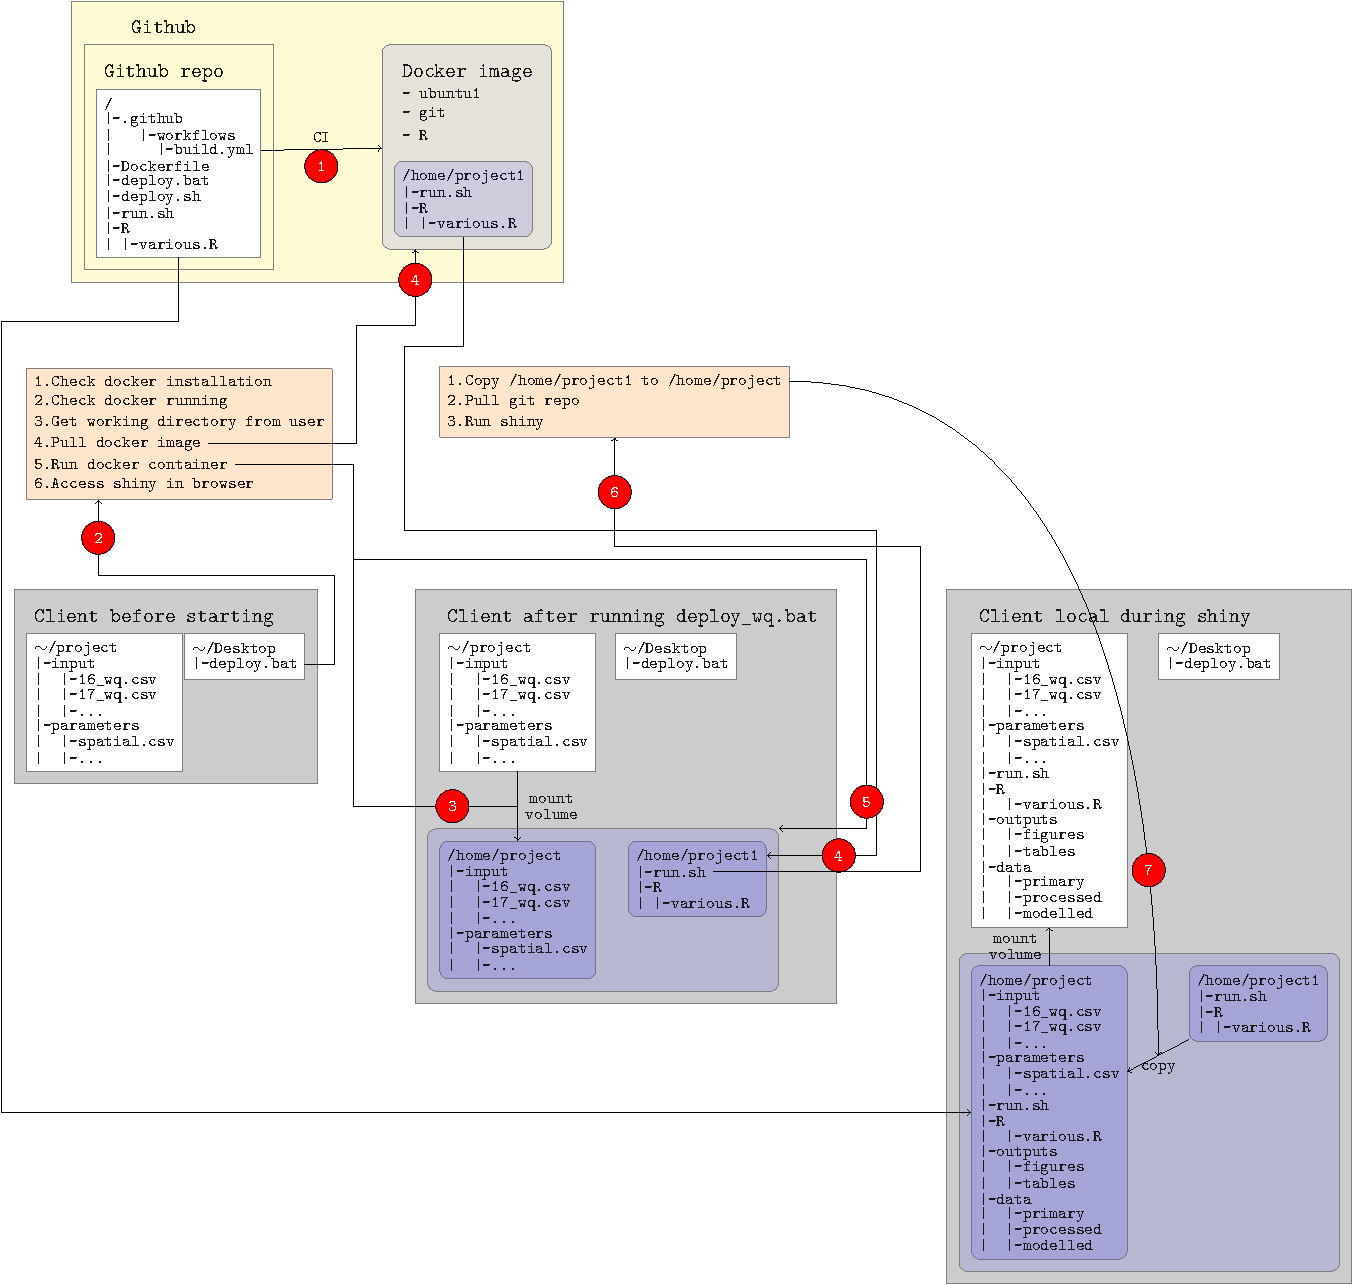
\includegraphics[keepaspectratio]{manual_files/figure-pdf/fig-diagram2-1.pdf}}

}

\caption{\label{fig-diagram2}Diagram illustrating the sequence of
filesystem events that occur during the development, deployment and
running of this app.}

\end{figure}%




\end{document}
